\subsection{Dịch vụ nhân vật (persona service)}

Mục đích: Chịu trách nhiệm quản lý hệ thống nhân vật (personas), kho giọng đọc (\texttt{Voices}), các nền tảng tổng hợp giọng nói (\texttt{TTS Engines}) và xử lý trực tiếp các yêu cầu chuyển đổi văn bản thành âm thanh (\texttt{Text-to-Speech}).

\begin{figure}[H]
\centering
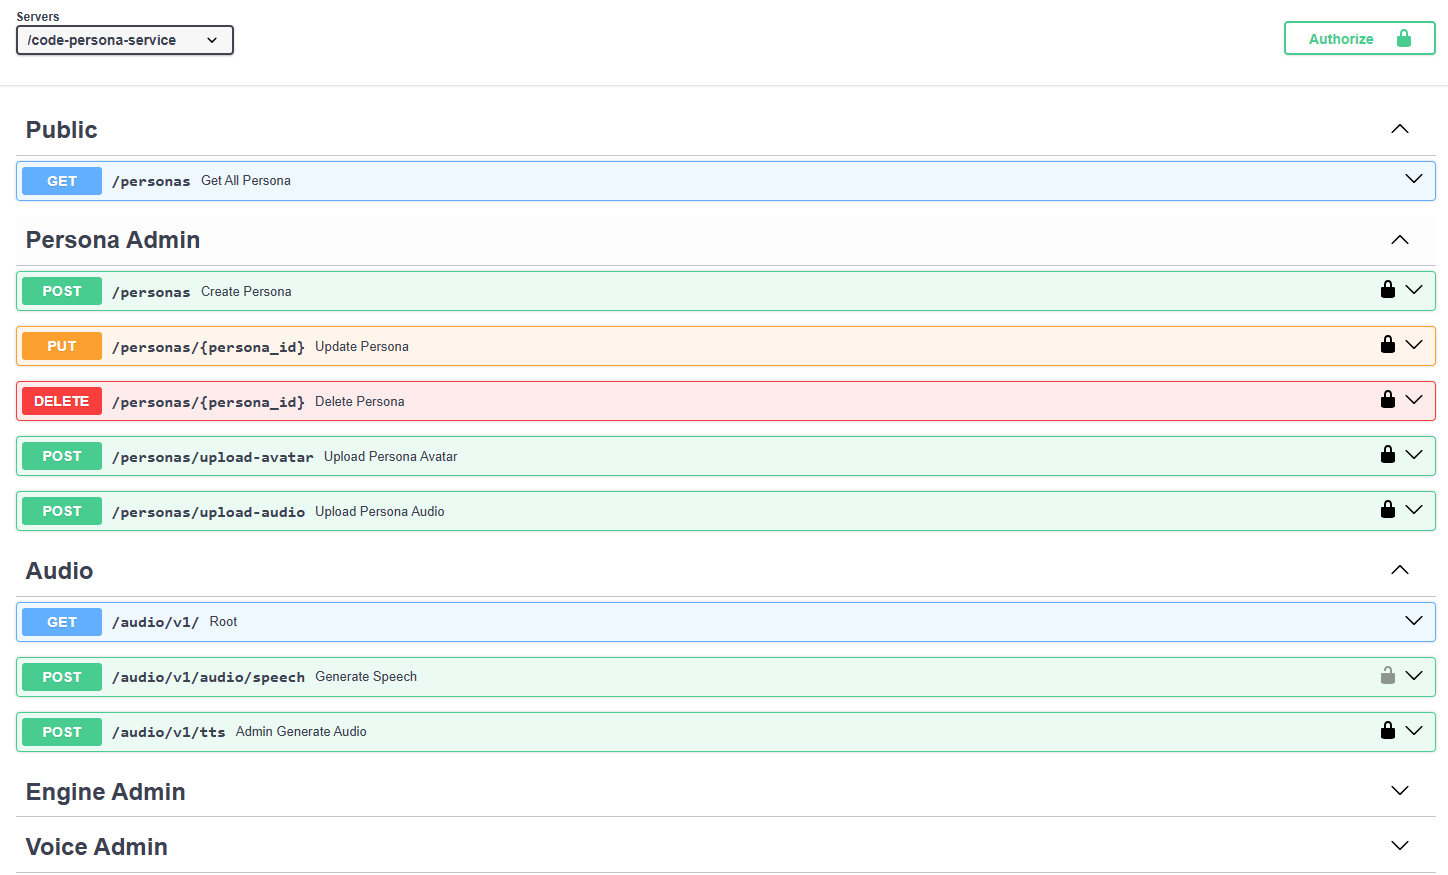
\includegraphics[width=0.85\textwidth]{pictures/persona-swagger2.png}
\caption{Tài liệu Swagger API Dịch vụ nhân vật}
\label{fig:persona-swagger}
\end{figure}

\subsubsection{Các chức năng chính}

\begin{itemize}
\item \textbf{Truy xuất danh sách nhân vật}:
\begin{itemize}
\item Cung cấp danh sách các nhân vật trong hệ thống, hỗ trợ phân trang và lọc theo \texttt{persona\_id}.
\end{itemize}

\item \textbf{Quản lý nhân vật (Dành cho ADMIN)}:
\begin{itemize}
\item Cho phép tạo mới, cập nhật thông tin hoặc xóa bỏ các nhân vật khỏi hệ thống.
\item Tải lên hình ảnh đại diện (\texttt{avatar}) và file âm thanh câu chào mẫu (welcome audio) cho từng nhân vật.
\end{itemize}

\item \textbf{Quản lý công cụ TTS (engines)}:
\begin{itemize}
\item Cho phép quản trị viên ADMIN định nghĩa, cập nhật, xóa và truy xuất danh sách các nền tảng dịch vụ cung cấp TTS.
\end{itemize}

\item \textbf{Quản lý giọng đọc (voices)}:
\begin{itemize}
\item Cho phép tạo, cập nhật, xóa và truy xuất danh sách các giọng đọc cụ thể, hỗ trợ bộ lọc theo công cụ/nền tảng.
\end{itemize}

\item \textbf{Đồng bộ ElevenLabs}:
\begin{itemize}
\item Tích hợp API đồng bộ danh sách giọng đọc mới nhất từ nhà cung cấp ElevenLabs trực tiếp về hệ thống cơ sở dữ liệu.
\end{itemize}

\item \textbf{Chuyển đổi Text-to-Speech}:
\begin{itemize}
\item Cung cấp chức năng tạo ra âm thanh từ văn bản đầu vào thông qua hai thư viện: \texttt{edge-tts} (tổng hợp online) và \texttt{piper-tts} (tổng hợp offline chất lượng cao).
\item Với \texttt{piper-tts}, hệ thống yêu cầu tệp mô hình giọng đọc được lưu trữ tại Cloudflare R2 và tự động tải xuống máy chủ cục bộ khi dịch vụ bắt đầu khởi động.
\end{itemize}

\item \textbf{Cơ chế Cache tối ưu (TTS Caching)}:
\begin{itemize}
\item \textbf{Disk Cache}: Sử dụng thư viện \texttt{diskcache} (cơ chế LRU, kích thước giới hạn 1GB) để lưu giữ các file âm thanh đã tổng hợp lên ổ đĩa. Các yêu cầu TTS trùng lặp nội dung sẽ được phản hồi tức thì, tiết kiệm băng thông và CPU.
\item \textbf{Memory Cache}: Lưu giữ các đối tượng mô hình Piper đã load vào bộ nhớ RAM (\texttt{\_loaded\_voices}), tránh việc phải nạp lại tệp tin mô hình \texttt{.onnx} nặng sau mỗi request, tối ưu tốc độ phát âm thanh.
\end{itemize}

\item \textbf{Lưu trữ tài nguyên}:
\begin{itemize}
\item Toàn bộ dữ liệu mẫu âm thanh (\texttt{audio}), hình ảnh (\texttt{images}) và mô hình (\texttt{models}) phục vụ cho dịch vụ nhân vật được lưu trữ an toàn tại Cloudflare R2.
\end{itemize}
\end{itemize}

Quản lý thư mục tài nguyên của dịch vụ nhân vật trên Cloudflare R2:

\begin{figure}[H]
\centering
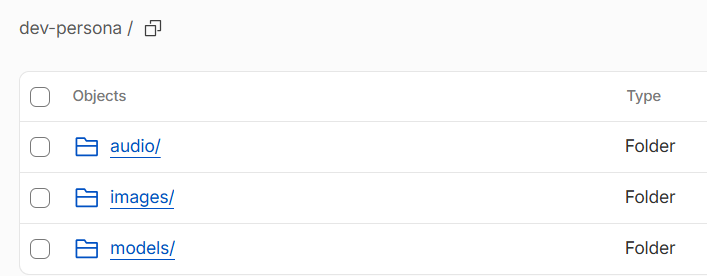
\includegraphics[width=0.85\textwidth]{pictures/r2per.png}
\caption{Tài nguyên nhân vật lưu trữ trên Cloudflare R2}
\label{fig:r2per}
\end{figure}

Quản lý migrations cơ sở dữ liệu của dịch vụ nhân vật:

\begin{figure}[H]
\centering
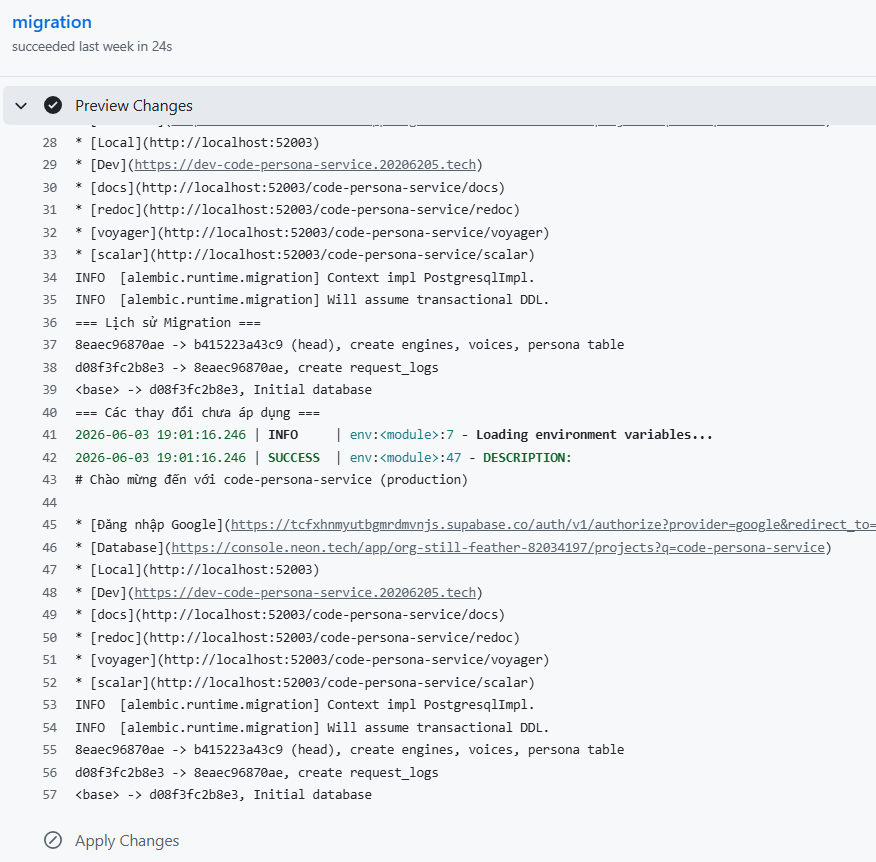
\includegraphics[width=0.85\textwidth]{pictures/persona-database-migration.png}
\caption{Quản lý migration cơ sở dữ liệu của dịch vụ nhân vật}
\label{fig:persona-database-migration}
\end{figure}

Cấu trúc các bảng trong cơ sở dữ liệu của Dịch vụ nhân vật:

\begin{figure}[H]
\centering
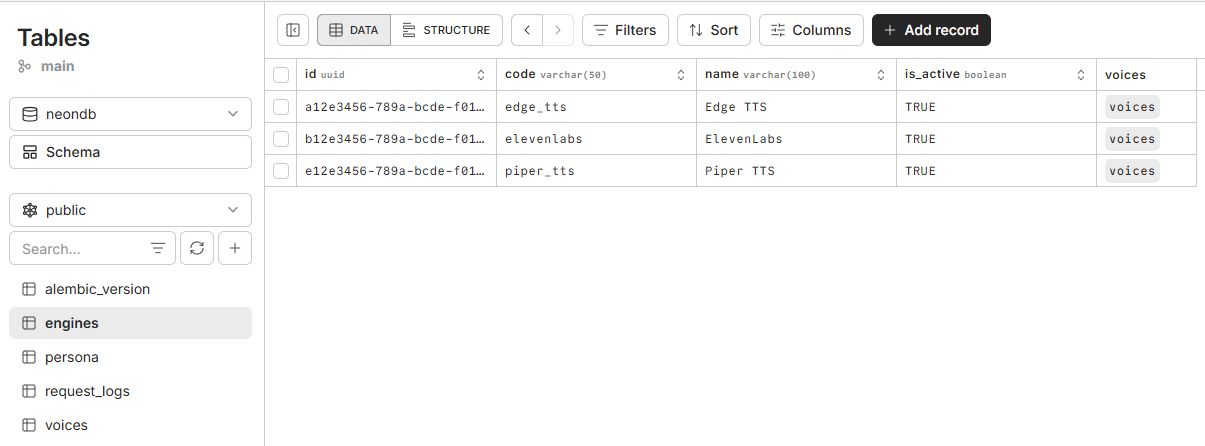
\includegraphics[width=0.85\textwidth]{pictures/persona-database.png}
\caption{Cấu trúc các bảng trong cơ sở dữ liệu của Dịch vụ nhân vật}
\label{fig:persona-database}
\end{figure}
